\documentclass[journal,12pt,twocolumn]{IEEEtran}
%
\usepackage{setspace}
\usepackage{gensymb}
%\doublespacing
\singlespacing

%\usepackage{graphicx}
%\usepackage{amssymb}
%\usepackage{relsize}
\usepackage[cmex10]{amsmath}
%\usepackage{amsthm}
%\interdisplaylinepenalty=2500
%\savesymbol{iint}
%\usepackage{txfonts}
%\restoresymbol{TXF}{iint}
%\usepackage{wasysym}
\usepackage{amsthm}
%\usepackage{iithtlc}
\usepackage{mathrsfs}
\usepackage{txfonts}
\usepackage{stfloats}
\usepackage{bm}
\usepackage{cite}
\usepackage{cases}
\usepackage{subfig}
%\usepackage{xtab}
\usepackage{longtable}
\usepackage{multirow}
%\usepackage{algorithm}
%\usepackage{algpseudocode}
\usepackage{enumitem}
\usepackage{mathtools}
\usepackage{steinmetz}
\usepackage{tikz}
\usepackage[american]{circuitikz}
\usepackage{verbatim}
\usepackage{tfrupee}
\usepackage[breaklinks=true]{hyperref}
%\usepackage{stmaryrd}
\usepackage{tkz-euclide} % loads  TikZ and tkz-base
\usetkzobj{all}
\usetikzlibrary{decorations.markings}
\usetikzlibrary{shapes.geometric}
\newif\iflabrev
\usepackage{listings}
    \usepackage{color}                                            %%
    \usepackage{array}                                            %%
    \usepackage{longtable}                                        %%
    \usepackage{calc}                                             %%
    \usepackage{multirow}                                         %%
    \usepackage{hhline}                                           %%
    \usepackage{ifthen}                                           %%
  %optionally (for landscape tables embedded in another document): %%
    \usepackage{lscape}     
\usepackage{multicol}
\usepackage{chngcntr}
%\usepackage{enumerate}

%\usepackage{wasysym}
%\newcounter{MYtempeqncnt}
\DeclareMathOperator*{\Res}{Res}
%\renewcommand{\baselinestretch}{2}
\renewcommand\thesection{\arabic{section}}
\renewcommand\thesubsection{\thesection.\arabic{subsection}}
\renewcommand\thesubsubsection{\thesubsection.\arabic{subsubsection}}

\renewcommand\thesectiondis{\arabic{section}}
\renewcommand\thesubsectiondis{\thesectiondis.\arabic{subsection}}
\renewcommand\thesubsubsectiondis{\thesubsectiondis.\arabic{subsubsection}}

% correct bad hyphenation here
\hyphenation{op-tical net-works semi-conduc-tor}
\def\inputGnumericTable{}                                 %%

\lstset{
%language=C,
frame=single, 
breaklines=true,
columns=fullflexible
}
%\lstset{
%language=tex,
%frame=single, 
%breaklines=true
%}

\begin{document}
%


\newtheorem{theorem}{Theorem}[section]
\newtheorem{problem}{Problem}
\newtheorem{proposition}{Proposition}[section]
\newtheorem{lemma}{Lemma}[section]
\newtheorem{corollary}[theorem]{Corollary}
\newtheorem{example}{Example}[section]
\newtheorem{definition}[problem]{Definition}
%\newtheorem{thm}{Theorem}[section] 
%\newtheorem{defn}[thm]{Definition}
%\newtheorem{algorithm}{Algorithm}[section]
%\newtheorem{cor}{Corollary}
\newcommand{\BEQA}{\begin{eqnarray}}
\newcommand{\EEQA}{\end{eqnarray}}
\newcommand{\define}{\stackrel{\triangle}{=}}
\bibliographystyle{IEEEtran}
%\bibliographystyle{ieeetr}
\providecommand{\mbf}{\mathbf}
\providecommand{\pr}[1]{\ensuremath{\Pr\left(#1\right)}}
\providecommand{\qfunc}[1]{\ensuremath{Q\left(#1\right)}}
\providecommand{\sbrak}[1]{\ensuremath{{}\left[#1\right]}}
\providecommand{\lsbrak}[1]{\ensuremath{{}\left[#1\right.}}
\providecommand{\rsbrak}[1]{\ensuremath{{}\left.#1\right]}}
\providecommand{\brak}[1]{\ensuremath{\left(#1\right)}}
\providecommand{\lbrak}[1]{\ensuremath{\left(#1\right.}}
\providecommand{\rbrak}[1]{\ensuremath{\left.#1\right)}}
\providecommand{\cbrak}[1]{\ensuremath{\left\{#1\right\}}}
\providecommand{\lcbrak}[1]{\ensuremath{\left\{#1\right.}}
\providecommand{\rcbrak}[1]{\ensuremath{\left.#1\right\}}}
\theoremstyle{remark}
\newtheorem{rem}{Remark}
\newcommand{\sgn}{\mathop{\mathrm{sgn}}}
\providecommand{\abs}[1]{\left\vert#1\right\vert}
\providecommand{\res}[1]{\Res\displaylimits_{#1}} 
\providecommand{\norm}[1]{\left\lVert#1\right\rVert}
%\providecommand{\norm}[1]{\lVert#1\rVert}
\providecommand{\mtx}[1]{\mathbf{#1}}
\providecommand{\mean}[1]{E\left[ #1 \right]}
\providecommand{\fourier}{\overset{\mathcal{F}}{ \rightleftharpoons}}
%\providecommand{\hilbert}{\overset{\mathcal{H}}{ \rightleftharpoons}}
\providecommand{\system}{\overset{\mathcal{H}}{ \longleftrightarrow}}
	%\newcommand{\solution}[2]{\textbf{Solution:}{#1}}
\newcommand{\solution}{\noindent \textbf{Solution: }}
\newcommand{\cosec}{\,\text{cosec}\,}
\providecommand{\dec}[2]{\ensuremath{\overset{#1}{\underset{#2}{\gtrless}}}}
\newcommand{\myvec}[1]{\ensuremath{\begin{pmatrix}#1\end{pmatrix}}}
\newcommand{\mydet}[1]{\ensuremath{\begin{vmatrix}#1\end{vmatrix}}}
%\numberwithin{equation}{section}
\numberwithin{equation}{subsection}
%\numberwithin{problem}{section}
%\numberwithin{definition}{section}
\makeatletter
\@addtoreset{figure}{problem}
\makeatother
\let\StandardTheFigure\thefigure
\let\vec\mathbf
%\renewcommand{\thefigure}{\theproblem.\arabic{figure}}
\renewcommand{\thefigure}{\theproblem}
%\setlist[enumerate,1]{before=\renewcommand\theequation{\theenumi.\arabic{equation}}
%\counterwithin{equation}{enumi}
%\renewcommand{\theequation}{\arabic{subsection}.\arabic{equation}}
\def\putbox#1#2#3{\makebox[0in][l]{\makebox[#1][l]{}\raisebox{\baselineskip}[0in][0in]{\raisebox{#2}[0in][0in]{#3}}}}
     \def\rightbox#1{\makebox[0in][r]{#1}}
     \def\centbox#1{\makebox[0in]{#1}}
     \def\topbox#1{\raisebox{-\baselineskip}[0in][0in]{#1}}
     \def\midbox#1{\raisebox{-0.5\baselineskip}[0in][0in]{#1}}
\vspace{3cm}
\title{
%	\logo{
Op-Amp Stability
%	}
}
\author{ Ritwik Sahani$^{*}$% <-this % stops a space
	\thanks{*The author is with the Department
		of Electrical Engineering, Indian Institute of Technology, Hyderabad
		502285 India. All content in this manual is released under GNU GPL.  Free and open source.}
	
}	
%\title{
%	\logo{Matrix Analysis through Octave}{\begin{center}\includegraphics[scale=.24]{tlc}\end{center}}{}{HAMDSP}
%}
% paper title
% can use linebreaks \\ within to get better formatting as desired
%\title{Matrix Analysis through Octave}
%
%
% author names and IEEE memberships
% note positions of commas and nonbreaking spaces ( ~ ) LaTeX will not break
% a structure at a ~ so this keeps an author's name from being broken across
% two lines.
% use \thanks{} to gain access to the first footnote area
% a separate \thanks must be used for each paragraph as LaTeX2e's \thanks
% was not built to handle multiple paragraphs
%
%\author{<-this % stops a space
%\thanks{}}
%}
% note the % following the last \IEEEmembership and also \thanks - 
% these prevent an unwanted space from occurring between the last author name
% and the end of the author line. i.e., if you had this:
% 
% \author{....lastname \thanks{...} \thanks{...} }
%                     ^------------^------------^----Do not want these spaces!
%
% a space would be appended to the last name and could cause every name on that
% line to be shifted left slightly. This is one of those "LaTeX things". For
% instance, "\textbf{A} \textbf{B}" will typeset as "A B" not "AB". To get
% "AB" then you have to do: "\textbf{A}\textbf{B}"
% \thanks is no different in this regard, so shield the last } of each \thanks
% that ends a line with a % and do not let a space in before the next \thanks.
% Spaces after \IEEEmembership other than the last one are OK (and needed) as
% you are supposed to have spaces between the names. For what it is worth,
% this is a minor point as most people would not even notice if the said evil
% space somehow managed to creep in.
% The paper headers
%\markboth{Journal of \LaTeX\ Class Files,~Vol.~6, No.~1, January~2007}%
%{Shell \MakeLowercase{\textit{et al.}}: Bare Demo of IEEEtran.cls for Journals}
% The only time the second header will appear is for the odd numbered pages
% after the title page when using the twoside option.
% 
% *** Note that you probably will NOT want to include the author's ***
% *** name in the headers of peer review papers.                   ***
% You can use \ifCLASSOPTIONpeerreview for conditional compilation here if
% you desire.
% If you want to put a publisher's ID mark on the page you can do it like
% this:
%\IEEEpubid{0000--0000/00\$00.00~\copyright~2007 IEEE}
% Remember, if you use this you must call \IEEEpubidadjcol in the second
% column for its text to clear the IEEEpubid mark.
% make the title area
\maketitle
\newpage
\tableofcontents
\bigskip
\renewcommand{\thefigure}{\theenumi}
\renewcommand{\thetable}{\theenumi}
%\renewcommand{\theequation}{\theenumi}
%\begin{abstract}
%%\boldmath
%In this letter, an algorithm for evaluating the exact analytical bit error rate  (BER)  for the piecewise linear (PL) combiner for  multiple relays is presented. Previous results were available only for upto three relays. The algorithm is unique in the sense that  the actual mathematical expressions, that are prohibitively large, need not be explicitly obtained. The diversity gain due to multiple relays is shown through plots of the analytical BER, well supported by simulations. 
%
%\end{abstract}
% IEEEtran.cls defaults to using nonbold math in the Abstract.
% This preserves the distinction between vectors and scalars. However,
% if the journal you are submitting to favors bold math in the abstract,
% then you can use LaTeX's standard command \boldmath at the very start
% of the abstract to achieve this. Many IEEE journals frown on math
% in the abstract anyway.
% Note that keywords are not normally used for peerreview papers.
%\begin{IEEEkeywords}
%Cooperative diversity, decode and forward, piecewise linear
%\end{IEEEkeywords}
% For peer review papers, you can put extra information on the cover
% page as needed:
% \ifCLASSOPTIONpeerreview
% \begin{center} \bfseries EDICS Category: 3-BBND \end{center}
% \fi
%
% For peerreview papers, this IEEEtran command inserts a page break and
% creates the second title. It will be ignored for other modes.
%\IEEEpeerreviewmaketitle
%\begin{abstract}
%This manual is an introduction to control systems in feedback circuits. Links to sample Python codes are available in the text.  
%\end{abstract}
%Download python codes using 
%\begin{lstlisting}
%svn co https://github.com/gadepall/school/trunk/control/feedback/codes
%\end{lstlisting}
%\section{Op-Amp RC Oscillator Circuits}
An op amp having a low-frequency gain of $10^{3}$ and a single-pole rolloff at $10^{4}$ rad/s is connected in a negative feedback loop via a feedback network having a transmission k and a two-pole rolloff at $10^{4}$ rad/s. Find the value of k above which the closed-loop amplifier becomes unstable.
\begin{enumerate}[label=\arabic*.,ref=\theenumi]

%\begin{enumerate}[label=\thesection.\arabic*.,ref=\thesection.\theenumi]
\numberwithin{equation}{enumi}
\renewcommand{\thefigure}{\theenumi.\arabic{figure}}

\item Find Open Loop Gain, $G(s)$\\
\solution Gain for an amplifier whose transfer function is characterised with a single pole is-
\begin{align}
    G(s) &= \frac{G_{o}}{1+ \frac{s}{w_{p}}}
\end{align}
Here, $G_{o}$ is low frequency gain and $w_{p}$ is pole frequency. Thus for our problem,
\begin{align}
\label{eq:olg}
    G(s) &= \frac{10^3}{1+\frac{s}{10^4}}
\end{align}

\item Find Feedback factor, $H(s)$\\
\solution Given transmission(=low freq. gain) and two pole roll-off at $10^4$rad/s.
\begin{align}
    H(s)&= \frac{k}{\left(1+\frac{s}{10^4}\right)^2}
\end{align}

\item Loop Gain, G(s)H(s)\\
\solution 
\begin{align}
    G(s)H(s) &= \frac{10^3k}{\left(1+\frac{s}{10^4}\right)^3}
\end{align}

\item Stability of the Closed Loop Amplifier\\
\solution Closed loop systems stability can be tested by examining the Gain Margin, or Phase Margin alternatively. First, let's find $\omega_{180}$, the phase cross-over frequency
\begin{align}
       \angle G(j\omega)H(j\omega) =  \angle\frac{10^3k}{\left(1+\frac{j\omega}{10^4}\right)^3}\\
       \implies -3tan^{-1}\left({\frac{\omega}{10^4}}\right)
\end{align}
At $\omega = \omega_{180}$,
\begin{align}
       -180^{\circ}= {-3tan^{-1}\left({\frac{\omega_{180}}{10^4}}\right)}\\
        \implies \omega_{180} = \sqrt{3}\times 10^4
\end{align}
For a stable system, $GM_{dB}<0$,
\begin{align}
    \implies \abs{G(j\omega_{180})H(j\omega_{180})}< 1 \\
    \implies \abs{\frac{10^3k}{\left(1-\sqrt{3}j\right)^3} } < 1\\
     \implies \frac{10^3\abs{k}}{8} < 1 \\
     \implies \abs{k} < 0.008
\end{align}

\item Analyze stability using phase margin.\\
\solution For a stable closed loop amplifier, phase(absolute value) at gain cross-over frequency($\omega_{1}$) must be less than $180\degree$ i.e. $PM>0$. Let's first find $\omega_{1}$.
\begin{align}
     \abs{G(j\omega_{1})H(j\omega_{1})}= 1  \\
   \implies \abs{\frac{10^3k}{{\sqrt{1+\frac{{\omega_{1}}^2}{10^8}}}^3}}=1\\
  \implies \omega_{1}=\sqrt{10^8\left(10^2k^{\frac{2}{3}}-1\right)}
\end{align}
For stability,
\begin{align}
  180^{\circ}>3tan^{-1}\left({\frac{\sqrt{10^8\left(10^2k^{\frac{2}{3}}-1\right)}}{10^4}}\right)\\
\end{align}
\begin{align}
  \implies \sqrt{10^8\left(10^2k^{\frac{2}{3}}-1\right)}&<\sqrt{3} \times 10^4\\
    \implies 10^2k^{\frac{2}{3}}&<4\\
\implies \abs{k}<0.008
\end{align}
Thus the closed loop amplifier is unstable for $k>0.008$.

\item Design the Feedback Circuit\\
\solution 
\begin{align}
    H(s)&= \frac{k}{\left(1+\frac{s}{10^4}\right)^2}\\
\label{eq:expeq}
    \implies k\left({\frac{1}{1+\frac{2s}{10^4}+\frac{s^2}{10^8}}}\right)  
\end{align}
To realise the transfer function above, consider the following circuit-

\begin{figure}[!ht]
	\begin{center}
		
		\resizebox{\columnwidth}{!}{\begin{circuitikz}
\ctikzset{bipoles/length=1cm}
\draw (-1,-0.5) node[]{} to [short](-1,0.5) to [short](0,0) to [short](-1,-0.5);
\draw 
(0,0) to[L =$L_2$,*-*] (2,0)to[R=$R_2$](4,0) to [C](4,-2.4) node[ground]{}
(-1,0)   to (-1.8,0)node at (-2,0){$V_0$}
(-0.75,0) node[]{k};
\draw node at (4.6,-1.2){$V_f$}
node at (4.6,0){$+$}
node at (4.6,-2.4){$-$}
node at (3.5,-1.2){$C_2$}
;\end{circuitikz}}
	\end{center}
\caption{Feedback Circuit}
\label{fig:ee18btech11038_feedb}
\end{figure}

Transfer function for the circuit in Fig \ref{fig:ee18btech11038_feedb} is,
\begin{align}
    k\left(\frac{\frac{1}{s{C_2}}}{{R_2}+s{L_2}+\frac{1}{s{C_2}}}\right)\\
    \implies k\left(\frac{1}{1+s{R_2}{C_2}+{s^2}{L_2}{C_2}}\right)
\end{align}

Comparing it with \ref{eq:expeq}, one possible set of values for $R_{2}$, $L_{2}$ and $C_{2}$ is-
\begin{align}
    R_{2}&= 2k\Omega \\
    L_{2}&= 100mH\\ 
C_{2}&= 100nF
\end{align}

\item Design the closed loop circuit.\\
\solution The closed loop circuit looks as shown in the Fig \ref{fig:ee18btech11038_cla}.

\begin{figure}[!ht]
	\begin{center}
		
		\resizebox{\columnwidth}{!}{\begin{circuitikz}
\ctikzset{bipoles/length=1cm}
\draw (0,-0.5) node[]{} to [short](0,0.5) to [short](1,0) to [short](0,-0.5);

\draw (0.3, 0) node{$k$};
\draw (1,0) to [R=$R_2$](3,0) to [L=$L_2$](5,0) to [C=$C_2$](5,-3) node[ground]{};
\draw (7.5,-0.35) node[op amp] (opamp_1){}
(opamp_1.-) -- (5,0)
(opamp_1.+) to[V=$V_i$](6.7,-3) node[ground]{}
(opamp_1.center) node{$10^3$}


(opamp_1.out) 
(8,-0.35) -- (11,-0.35)--(11,-4)--(-0.8,-4)to (-0.75,0) --(0,0)
(11,-0.35) to (11.5,-0.35)node at (11.8,-0.35){$V_0$}

(5,0)--(5,0.2)node at (5,0.5){$V_f$};
\end{circuitikz}}
	\end{center}
\caption{Closed Loop Circuit}
\label{fig:ee18btech11038_cla}
\end{figure}

Here, the op-amp has a gain given by
\begin{align}
    G(s) &= \frac{10^3}{1+\frac{s}{10^4}}
\end{align}
\item Find the closed loop transfer function, $T(s)$.\\
\solution 
\begin{align}
    T(s)&=\frac{\frac{10^3}{1+\frac{s}{10^4}}}{1+\frac{10^3k}{\left(1+\frac{s}{10^4}\right)^3}}\\
    &=\frac{10^7s^2+2\times10^{11}s+10^{15}}{s^3+3\times10^4s^2+3\times10^8s+10^{12} + 10^{15}\times k}
\end{align}

\item Sketch the bode plot of T(s).\\
\solution Assuming $k=0.001$ for numerical simplicity.
The bode plot looks as shown in Fig \ref{fig:ee18btech11038_bode}
You can find the python script used to generate the bode plot here:
\begin{lstlisting}
spice/ee18btech11038_bode.py
\end{lstlisting}
\begin{figure}[!ht]
\centering
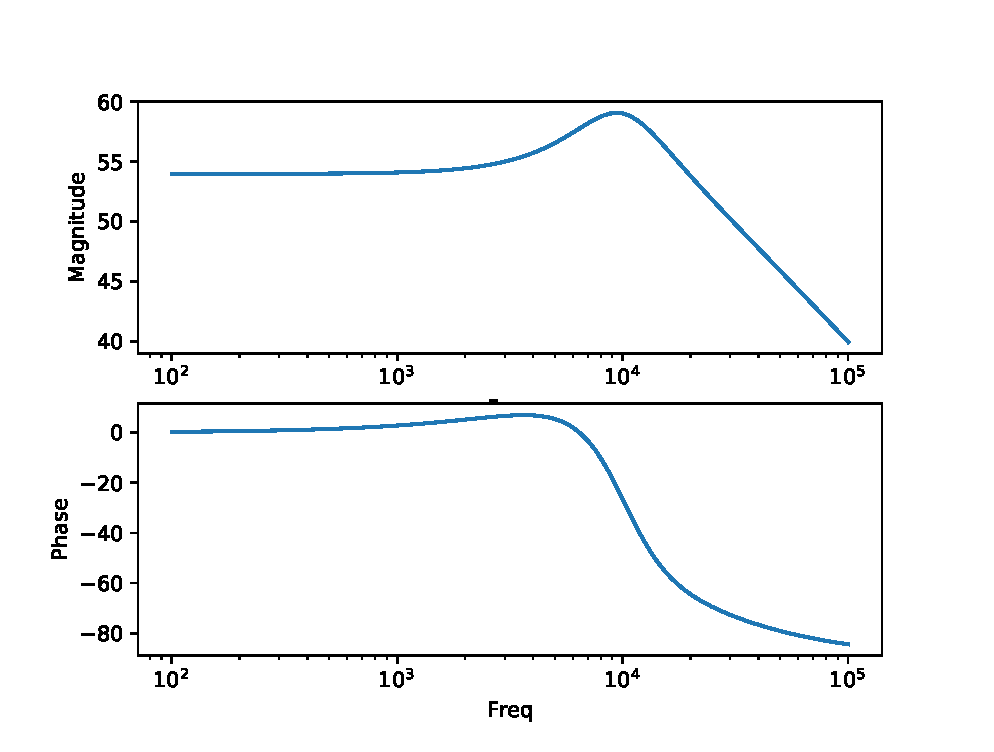
\includegraphics[width=\columnwidth]{./figs/ee18btech11038_bode.eps}
\caption{Bode Plot for $T(s)$}
\label{fig:ee18btech11038_bode}
\end{figure}

\item Simulate the circuit using spice.\\
\solution For simulation purpose, we will realise the closed loop amplifier as shown in Fig \ref{fig:ee18btech11038_sim} in spice.


\begin{figure}[!ht]
	\begin{center}
		
		\resizebox{\columnwidth}{!}{\begin{circuitikz}
\ctikzset{bipoles/length=1cm}
\draw (0,-0.5) node[]{} to [short](0,0.5) to [short](1,0) to [short](0,-0.5);

\draw (0.3, 0) node{$k$};
\draw (1,0) to [R=$R_2$](3,0) to [L=$L_2$](5,0) to [C=$C_2$](5,-3) node[ground]{};
\draw (5,0) to[short, -o] (6.5,0)node[right]{$v_{f}$};
\draw (6.5, -2)  to[vsource, l=$v_{i}$](6.5, -3) to node[ground]{}(6.5,-3);
\draw (6.5,-2) to[short, -o] (6.5,-1.5)node[right]{$v_{i}$};
\draw (6.5,0)node[below]{$-$};
\draw (6.5,-1.5)node[above]{$+$};
\draw (8, 0) to[cV, l =$10^3\times(v_{i}-v_{f})$](8,-2) to node[ground]{}(8,-2);
\draw (8,0) to [L = $L_{1}$ ](11.5,0) to [R=$R_{1}$](11.5,-2) to node[ground]{}(11.5,-2);
\draw (11.5,0) to[short, -o] (13,0)node[right]{$v_{o}$};
\draw (12.5, 0) to[short](12.5,-4) to[short](-1,-4) to[short](-1,0) to[short](0,0);
\end{circuitikz}}
	\end{center}
\caption{Circuit used for Simulation}
\label{fig:ee18btech11038_sim}
\end{figure}

\begin{align}
    R_{1}&= 1k\Omega \\
    L_{1}&= 100mH
\end{align}

\item Verify by results obtained using simulation\\
\solution Fig \ref{fig:ee18btech11038_freqres} shows the frequency response plot for the circuit in Fig \ref{fig:ee18btech11038_freqres} obtained using an A.C. sweep in spice.
You can find the netlist for the simulated circuit here:
\begin{lstlisting}
spice/ee18btech11038_opamp.cir
\end{lstlisting}
You can find the python script used to generate the output here:
\begin{lstlisting}
spice/ee18btech11038_opamp.py
\end{lstlisting}
\begin{figure}[!ht]
\centering
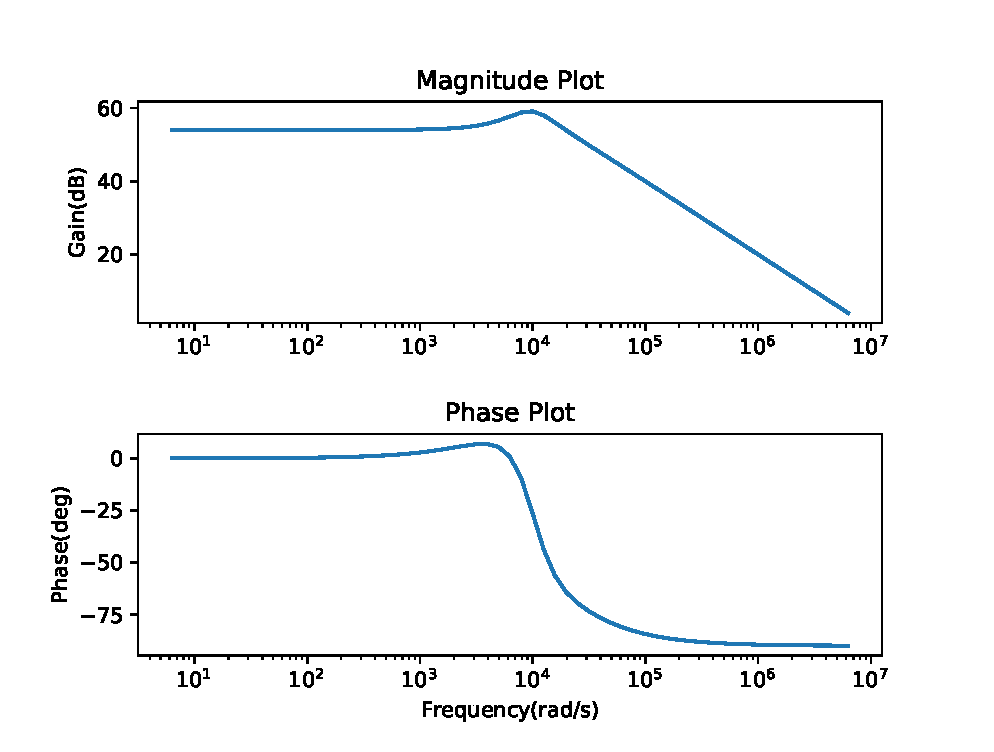
\includegraphics[width=\columnwidth]{./figs/ee18btech11038_freqres.eps}
\caption{Frequency Response from Simulation}
\label{fig:ee18btech11038_freqres}
\end{figure}

Clearly, the bode plot in Fig \ref{fig:ee18btech11038_bode} and plots in Fig \ref{fig:ee18btech11038_freqres} match. Hence verified.











\end{enumerate}



\end{document}